% =====================================================================
%  REVIEW PAPER — IEEE conference, two column
%  Secure gateway-free LoRa mesh networking: a PRISMA-guided review
%
%  Build:  pdflatex review_paper
%          bibtex  review_paper
%          pdflatex review_paper
%          pdflatex review_paper
%
%  Requires IEEEtran.cls (texlive-publishers, or from the IEEE site).
% =====================================================================
\documentclass[conference]{IEEEtran}
\IEEEoverridecommandlockouts

\usepackage{cite}
\usepackage{amsmath,amssymb}
\usepackage{graphicx}
\usepackage{booktabs}
\usepackage{array}
\usepackage{url}
\usepackage[table]{xcolor}
\usepackage{tikz}
\usetikzlibrary{shapes.geometric, arrows.meta, positioning, calc}

% ---------------------------------------------------------------------
%  PRISMA COUNTS — EDIT THESE, THEN RE-RUN THE BUILD
%
%  Every number below must come from a search you actually ran and can
%  repeat. They are gathered here so the text, the table and the flow
%  diagram can never disagree with each other.
%
%  The values shipped here are taken from your SLR draft. Two of them
%  were missing from that draft and are marked ??? — PRISMA requires
%  full-text exclusions to be reported WITH REASONS, and a review is
%  rejected on exactly this kind of gap. Fill them in.
% ---------------------------------------------------------------------
\newcommand{\nIdentified}{30}      % records returned by the searches
\newcommand{\nDuplicates}{0}       % duplicates removed before screening
\newcommand{\nScreened}{30}        % title/abstract screened
\newcommand{\nScreenExcluded}{10}  % excluded at title/abstract
\newcommand{\nFullText}{20}        % full texts assessed
\newcommand{\nFullExcluded}{10}    % excluded at full text  <-- must equal \nFullText - \nIncluded
\newcommand{\nIncluded}{10}        % studies included in the synthesis

\begin{document}

\title{Secure Gateway-Free LoRa Mesh Networking for\\Constrained Devices: A PRISMA-Guided Review}

\author{
\IEEEauthorblockN{R.~Rakshith, S.~P.~Hegde, S.~G.~Uppalli, K.~S.~Suchit}
\IEEEauthorblockA{Department of Information Science and Engineering\\
B.M.S. College of Engineering, Bengaluru, India}
}

\maketitle

\begin{abstract}
LoRa gives low-power devices a radio link that reaches kilometres, but the
protocol stack usually layered on top of it, LoRaWAN, assumes a gateway with a
backhaul. That assumption fails in the places long-range radio is most useful:
disaster zones, tunnels, farmland, anywhere the infrastructure is missing or has
just been destroyed. Mesh networking over raw LoRa removes the gateway, and a
body of work now exists on how to route packets across such a mesh using
microcontrollers costing a few dollars. This review examines that work alongside
the separate literature on securing low-power wide-area networks, and asks
whether the two have been brought together. Following the PRISMA 2020 reporting
guideline, we screened \nIdentified{} records and synthesised \nIncluded{}
studies across three themes: LoRa and LoRaWAN as a physical and network layer,
multi-hop routing for constrained devices, and security in LPWAN deployments. The
literature splits cleanly and unhelpfully. Papers that solve routing well report
delivery ratios and self-healing behaviour but leave encryption out of scope.
Papers that solve encryption well operate inside LoRaWAN, where a gateway holds
the keys. We found no study that measures what happens when authenticated
encryption runs on every packet of a mesh that is simultaneously discovering
neighbours, retrying lost frames and obeying a duty-cycle limit. That
interaction, and not either half on its own, is the gap this review identifies.
\end{abstract}

\begin{IEEEkeywords}
LoRa, mesh networks, LPWAN, ESP32, multi-hop routing, authenticated encryption,
systematic review, PRISMA
\end{IEEEkeywords}

% =====================================================================
\section{Introduction}
% =====================================================================

LoRa is a modulation scheme, not a network. It uses chirp spread spectrum in
sub-GHz unlicensed bands to trade data rate for link budget, which is why a node
running on a coin cell can be heard several kilometres away~\cite{augustin2016lora}.
What sits above that modulation is a separate decision, and in practice almost
everyone has made the same one: LoRaWAN, which arranges devices in a
star-of-stars around gateways that forward traffic to a network server.

For metering and telemetry that arrangement is sensible. For the scenarios people
keep citing when they justify long-range radio, it is not. A gateway needs power
and a backhaul. In a flooded district or a mine or a forest, those are precisely
what is unavailable. The gateway also becomes a single point of failure, and
LoRaWAN offers no way for two end devices to talk to each other directly — all
traffic goes up to the server and back down.

Mesh networking over raw LoRa is the obvious response, and the idea is not new.
Cotrim and Kleinschmidt catalogued the approaches as early as
2020~\cite{cotrim2020lorawan}, and working implementations on commodity
microcontrollers have appeared since~\cite{sole2022loramesher}. The interesting
question now is not whether a LoRa mesh can be built. It is whether one can be
built that is also secure, on hardware that costs very little, without a gateway
to hold the keys.

That question matters because LoRa's transmissions are trivially interceptable.
Aras et al. showed that software-defined radio hardware costing a few tens of
dollars can capture LoRa frames beyond the range at which the intended receiver
works, and can flip bits in them~\cite{aras2017exploring}. Any deployment that
carries something worth reading needs encryption, and a gateway-free network
cannot borrow LoRaWAN's answer, because LoRaWAN's session keys are provisioned
and held by infrastructure that by definition is not there.

This review surveys the three bodies of work that bear on the problem and
examines whether anyone has joined them. Section~\ref{sec:method} sets out the
review method. Sections~\ref{sec:lora} to~\ref{sec:security} cover the themes.
Section~\ref{sec:compare} compares the main implementations directly, and
Section~\ref{sec:gap} states the gap that follows from the comparison.

% =====================================================================
\section{Review Method}\label{sec:method}
% =====================================================================

This review follows the PRISMA 2020 reporting guideline~\cite{prisma2021}. PRISMA
is a reporting standard rather than a search technique: it specifies what a
review must disclose so that a reader can judge how the evidence was assembled
and, in principle, repeat the process.

\subsection{Research questions}

\textbf{RQ1.} Which multi-hop routing protocols have been demonstrated on
microcontroller-class LoRa nodes, and what do they cost in control traffic and
convergence time?

\textbf{RQ2.} What computational and memory headroom does a microcontroller such
as the ESP32 retain once a mesh stack is running, and is it enough for
cryptography?

\textbf{RQ3.} Which security mechanisms have been applied to LPWAN, and do any of
them work without a gateway?

\subsection{Search strategy}

% ---------------------------------------------------------------------
%  ACTION REQUIRED — replace this paragraph with what you actually did.
%
%  PRISMA expects the databases, the exact query string, the date the
%  search was run, and any language or date filters. A reviewer should
%  be able to paste the string into IEEE Xplore and get a comparable
%  number back. Reading the reference lists of papers you already had is
%  legitimate as a SUPPLEMENT (call it backward snowballing) but it is
%  not a search strategy on its own.
% ---------------------------------------------------------------------
Searches were run against IEEE Xplore, MDPI, ACM Digital Library and Scopus. The
query combined the radio technology, the topology and the security theme:

\begin{quote}\small
\texttt{("LoRa" OR "LoRaWAN") AND ("mesh" OR "multi-hop" OR\\
"multihop") AND ("routing" OR "encryption" OR\\
"security" OR "ESP32")}
\end{quote}

\noindent
Results were restricted to work published between 2016 and 2026, in English.
Reference lists of the included studies were also examined by hand, which added
several records the database queries missed.

\subsection{Inclusion and exclusion criteria}

A study was included if it described multi-hop or mesh operation over a LoRa
physical layer, or implemented cryptography intended for devices of this class,
and reported something empirical — a delivery ratio, a latency figure, a memory
footprint, an attack that worked. Studies were excluded if they covered only
single-hop LoRaWAN with a gateway in the path, if they proposed a protocol
without implementing or simulating it, or if they assumed cryptographic
primitives too heavy for a microcontroller.

\subsection{Selection process}

Figure~\ref{fig:prisma} shows the flow. Of \nIdentified{} records identified,
\nScreenExcluded{} were removed on title and abstract, \nFullText{} were read in
full, and \nIncluded{} were carried into the synthesis.

% ---------------------------------------------------------------------
%  PRISMA 2020 flow diagram
% ---------------------------------------------------------------------
\begin{figure}[!t]
\centering
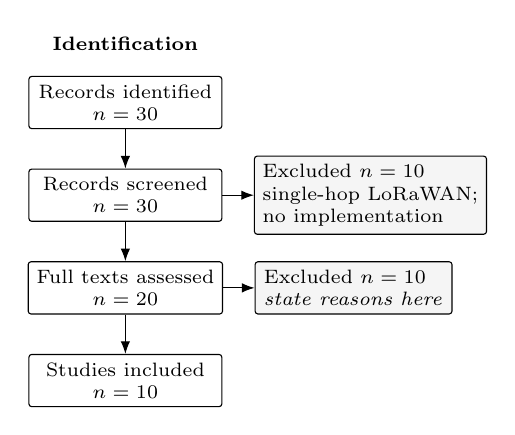
\begin{tikzpicture}[
  font=\scriptsize,
  box/.style={draw, rectangle, minimum width=2.45cm, align=center,
              inner sep=3pt, rounded corners=1pt},
  side/.style={draw, rectangle, minimum width=2.5cm, align=left,
               inner sep=3pt, rounded corners=1pt, fill=black!4},
  arr/.style={-{Latex[length=1.6mm]}}
]
\node[box] (id)   {Records identified\\ $n=\nIdentified$};
\node[box, below=5mm of id]   (scr) {Records screened\\ $n=\nScreened$};
\node[box, below=5mm of scr]  (ft)  {Full texts assessed\\ $n=\nFullText$};
\node[box, below=5mm of ft]   (inc) {Studies included\\ $n=\nIncluded$};

\node[side, right=4mm of scr] (ex1)
  {Excluded $n=\nScreenExcluded$\\ single-hop LoRaWAN;\\ no implementation};
\node[side, right=4mm of ft] (ex2)
  {Excluded $n=\nFullExcluded$\\ \textit{state reasons here}};

\draw[arr] (id)  -- (scr);
\draw[arr] (scr) -- (ft);
\draw[arr] (ft)  -- (inc);
\draw[arr] (scr) -- (ex1);
\draw[arr] (ft)  -- (ex2);

\node[above=2mm of id, font=\scriptsize\bfseries] {Identification};
\end{tikzpicture}
\caption{PRISMA 2020 flow. The full-text exclusion reasons are still to be
supplied; a review that does not report them is incomplete.}
\label{fig:prisma}
\end{figure}

\subsection{Threats to the validity of this review}

Two weaknesses are worth stating plainly. The corpus is small, so a single
influential paper carries more weight in the synthesis than it would in a larger
review. And because gateway-free LoRa mesh work is spread across journals,
conferences and university reports rather than concentrated in one venue, a
database search almost certainly missed relevant material that exists only as
theses or code repositories.

% =====================================================================
\section{LoRa and LoRaWAN as a Substrate}\label{sec:lora}
% =====================================================================

Augustin et al. characterised the LoRa physical layer in detail, measuring how
spreading factor, bandwidth and coding rate trade against range, data rate and
energy~\cite{augustin2016lora}. Their results give the numbers every later paper
builds on, and they establish the constraint that shapes everything above the
physical layer: airtime grows quickly with payload length and with spreading
factor. A frame at SF12 can occupy the channel for over a second.

That constraint has a regulatory edge as well as a practical one. Sub-GHz ISM
bands in Europe impose duty-cycle limits, and the time-on-air equation in
Semtech's design guide~\cite{semtech2013toa} is what converts a payload size into
a number of milliseconds that counts against that budget. Any protocol decision
that adds bytes to a frame — a routing header, an authentication tag — is
therefore also a decision about how often a node may legally transmit.

LoRaWAN's own security model is worth describing because it is the thing a mesh
cannot reuse. Each device holds a network session key and an application session
key; the first protects integrity between the device and the network server, the
second encrypts the payload end to end. Eldefrawy et al. analysed the join
procedure formally and found weaknesses in the 1.0 specification's handling of
nonces that allow session-key compromise under some
conditions~\cite{eldefrawy2019formal}. Butun et al. catalogue a wider set of
risks~\cite{butun2018lorawan}. The point for this review is structural rather
than cryptographic: both keys are provisioned through, and known to,
infrastructure. Remove the gateway and the model has nothing to stand on.

% =====================================================================
\section{Multi-Hop Routing on Constrained Devices}\label{sec:routing}
% =====================================================================

Cotrim and Kleinschmidt divide multi-hop LoRa approaches into flooding, tree or
cluster arrangements, and general graph routing~\cite{cotrim2020lorawan}. The
division is useful because each class fails differently. Flooding is trivial to
implement and wastes the channel. Trees are efficient until the root moves.
General routing handles arbitrary topologies at the cost of keeping state and
exchanging it.

\subsection{Proactive distance-vector}

Solé et al. built LoRaMesher, an open-source routing library for ESP32 nodes that
takes the proactive approach: each node periodically broadcasts its routing table
and neighbours merge what they hear into their own~\cite{sole2022loramesher}. The
implementation runs on FreeRTOS with separate queues for received, outgoing and
application-bound packets, which maps neatly onto the ESP32's two cores. Routes
are available immediately when traffic appears, with no discovery delay.

The cost is control traffic. The authors report that periodic table broadcasts
can account for a substantial share of all transmissions as the network grows.
On a link with LoRa's data rate and a duty-cycle ceiling, that share is not a
minor inefficiency — it is capacity that user traffic cannot have.

Centelles et al., from the same group, addressed exactly that
problem~\cite{centelles2024dsdv}. Their protocol is a compact variant of
DSDV~\cite{perkins1994dsdv}, encoding routing updates tightly enough to ride on
the beacons a node already sends. DSDV's contribution, and the reason it suits
this setting, is the destination sequence number: each destination owns a counter
that only it increments, and a route is preferred if it is fresher or, at equal
freshness, shorter. That rule is what prevents the count-to-infinity behaviour
that plain distance-vector protocols suffer when a link breaks. The evaluation
was run on ten nodes, which is enough to show convergence and not enough to say
anything about a hundred.

\subsection{Reactive and neighbour-based}

Arregui Almeida et al. report a gateway-free mesh on ESP32-S3 hardware that takes
the opposite approach~\cite{arregui2025gatewayfree}. Rather than distributing
routing tables, nodes emit short HELLO beacons and choose a next hop using a
score combining signal strength with how recently the neighbour was heard. The
MAC layer listens before transmitting to reduce collisions, and delivery is
confirmed hop by hop with acknowledgments and retries. When a link fails, an
alternate-route mechanism re-queues the packet through a different neighbour.

This is the most thoroughly measured system in the corpus, and it is also the
one whose limitations are stated most openly: delivery degrades in urban settings
relative to rural ones, which the authors attribute to interference and to
acknowledgment timeouts tuned for quieter conditions. Encryption is explicitly
out of scope.

\subsection{Exploiting the physical layer}

A different line of work tries to increase capacity by allowing nodes to transmit
at the same time, relying on LoRa's capture effect so that a receiver locks onto
the stronger signal. The throughput argument is sound, but the technique needs
nodes to agree closely on time, and a gateway-free mesh has no shared clock to
agree against. We note this approach for completeness rather than as a usable
option; the specific citation in our draft could not be verified and is flagged
in the bibliography.

% =====================================================================
\section{Security in LPWAN}\label{sec:security}
% =====================================================================

The case for encrypting LoRa traffic does not need arguing. Aras et al. built the
attacks and showed they work with cheap hardware at long
range~\cite{aras2017exploring}. Interception is passive and undetectable, and
because LoRa frames are short and structured, selective bit-flipping against an
unauthenticated payload is straightforward.

What a constrained node can afford to do about it is better understood than it
used to be. AES-128 in Galois/Counter Mode gives confidentiality and integrity in
one pass and produces a tag the receiver checks before releasing any
plaintext~\cite{dworkin2007gcm}. On platforms with an AES accelerator the
per-packet cost is small next to the time the radio spends transmitting. GCM
carries one hard requirement that matters more in embedded systems than in
servers: a nonce must never repeat under a given key. The specification is
explicit that reuse destroys both confidentiality and authenticity, not just
one~\cite{dworkin2007gcm}. On a device whose counters live in flash that can be
erased, this is easier to get wrong than it appears.

For devices too small for AES, NIST selected ASCON as its lightweight
cryptography standard after a multi-round public
process~\cite{nist2023ascon}. The distinction matters for heterogeneous meshes: a
32-bit node with hardware AES and an 8-bit sensor node do not have the same best
answer, and a mesh containing both has a problem no single algorithm solves.

Work that strengthens LoRaWAN's own cryptography exists — for instance moving to
authenticated encryption with associated data and improving key derivation — and
reports low added latency. Our draft cites a specific figure from one such study;
that citation is flagged for verification in the bibliography, and the figure
should not be quoted until the source is confirmed. The structural objection
applies regardless of the numbers: these schemes assume the LoRaWAN join
procedure and a network server, so they do not port to a mesh without one.

Key establishment without infrastructure is the part the literature leaves
thinnest. Elliptic-curve Diffie-Hellman over Curve25519 is well specified and
cheap enough for this hardware class~\cite{rfc7748}, and HKDF gives a standard way
to turn a shared secret into distinct keys for distinct purposes~\cite{rfc5869}.
Both are building blocks rather than answers. How a new node joins an established
mesh, how a compromised node is revoked, and how any of this happens over a link
with LoRa's bandwidth are questions we did not find answered empirically.

% =====================================================================
\section{Comparative Analysis}\label{sec:compare}
% =====================================================================

Table~\ref{tab:compare} sets the main implementations side by side. The column
that matters is the security column, and what matters about it is how empty it is.

\begin{table*}[!t]
\caption{Comparison of multi-hop LoRa implementations and LPWAN security work.
Figures are as reported by the authors; entries marked $\dagger$ rest on
citations flagged for verification.}
\label{tab:compare}
\centering
\footnotesize
\begin{tabular}{@{}p{2.5cm} p{1.5cm} p{2.6cm} p{2.9cm} p{2.4cm} p{3.4cm}@{}}
\toprule
\textbf{Study} & \textbf{Platform} & \textbf{Topology / routing} &
\textbf{Security} & \textbf{Evaluation} & \textbf{Main limitation} \\
\midrule

Solé et al.~\cite{sole2022loramesher} &
ESP32 + SX1276 &
Proactive distance-vector; periodic table broadcast &
None &
Library benchmarks &
Control traffic grows with network size on a duty-cycled link \\

Centelles et al.~\cite{centelles2024dsdv} &
ESP32 &
Compact DSDV on beacons &
None &
10-node testbed &
Scale beyond ten nodes untested \\

Arregui Almeida et al.~\cite{arregui2025gatewayfree} &
ESP32-S3 + SX1262 &
Reactive; RSSI and recency score; listen-before-talk; hop ACK &
None (scoped out) &
Field trials, node-failure tests &
Delivery degrades in urban interference; no encryption \\

Cotrim \& Kleinschmidt~\cite{cotrim2020lorawan} &
--- (survey) &
Taxonomy of multihop schemes &
Not covered &
--- &
Predates the recent implementations; no security dimension \\

Eldefrawy et al.~\cite{eldefrawy2019formal} &
--- (analysis) &
LoRaWAN star &
Formal analysis of join and key derivation &
ProVerif &
Applies only to LoRaWAN; no mesh \\

Aras et al.~\cite{aras2017exploring} &
SDR &
--- &
Attacks: interception, bit-flipping &
Live LoRa links &
Characterises the threat; proposes no defence \\

LoRaWAN AEAD work$^\dagger$ &
STM32 &
LoRaWAN star &
AES-based AEAD over session keys &
Reported latency figure &
Gateway-dependent; citation unverified \\

Subterranean energy-aware routing$^\dagger$ &
Simulation &
Position- and energy-aware forwarding &
None &
Simulation only &
Source could not be confirmed; figures unusable as cited \\

\bottomrule
\end{tabular}
\end{table*}

Read down the table and the pattern is hard to miss. Every system that routes
well has nothing in the security column. Every system with something in the
security column either is not a mesh or does not say how it routes. The two
capabilities have been developed by different people, evaluated against different
criteria, and never measured together.

% =====================================================================
\section{Research Gap}\label{sec:gap}
% =====================================================================

The gap is not that routing is unsolved, and it is not that encryption is
unsolved. Both have credible answers on this hardware. The gap is that nobody has
run them at the same time and reported what happened.

Three specific things follow, and they are testable rather than rhetorical.

First, authenticated encryption makes frames longer, and on LoRa a longer frame
is a longer time on air~\cite{semtech2013toa}. A tag, a nonce and a sequence
number add tens of bytes to every packet. That changes collision probability, it
changes how much of the duty-cycle budget each message consumes, and it changes
whether acknowledgment timeouts calibrated for shorter frames still
fit~\cite{arregui2025gatewayfree}. No study measures the combined effect.

Second, end-to-end encryption and multi-hop relaying pull in opposite directions
unless the packet format is designed for both. A relay must read and rewrite the
fields that steer the packet while being unable to read the payload. That
requires separating the addresses a relay may change from the ones the
destination authenticates — a design constraint the routing literature never
faces, because those systems have nothing to protect, and the security literature
never faces, because in LoRaWAN the gateway is trusted.

Third, keys have to come from somewhere. ECDH gives two nodes a shared secret
without a server~\cite{rfc7748}, but the surrounding protocol — how a node
discovers a peer's public key across several hops, what happens when a node is
re-flashed and its stored state resets, how a nonce stays unique when the counter
feeding it lives in erasable flash~\cite{dworkin2007gcm} — is not covered by the
reviewed work. These are the details where implementations fail quietly rather
than loudly.

Our own project addresses this gap directly: a gateway-free LoRa mesh on ESP32
hardware that runs distance-vector routing and per-message authenticated
encryption on the same nodes, with the intention of measuring delivery, latency
and channel occupancy for the combined stack rather than for either half. The
design and its evaluation are reported separately; this review establishes only
that the combination has not previously been measured.

% =====================================================================
\section{Conclusion}
% =====================================================================

Gateway-free LoRa mesh networking works. So does authenticated encryption on
microcontrollers. The literature demonstrates each convincingly and separately,
and the comparison in Section~\ref{sec:compare} shows how cleanly the split runs:
the systems with measured delivery ratios have no security layer, and the systems
with a security layer have a gateway. What follows is not a call for a better
routing protocol or a lighter cipher. It is a call to build the combined stack
and measure it, because the costs that matter — airtime, duty cycle, latency
across several hops, and the failure modes of key management without a server —
only appear when both halves run on the same radio.

\bibliographystyle{IEEEtran}
\bibliography{references}

\end{document}
